\section{Schottky groups}\label{sec:schottky}

A M\"obius transformation $z \mapsto (\alpha z + \beta)/(\gamma z + \delta)$,
with $\alpha\delta - \beta\gamma \ne 0$, is a bijection of the Riemann sphere
$\widehat{\C} = \C \cup \{\infty\}$ that takes circles and lines to circles
and lines. Let $D_a$, $D_{a^{-1}}$, $D_b$, $D_{b^{-1}}$ be open round discs in
$\C$ whose closures are pairwise disjoint.

Given a target disc $D$ (center $c$, radius $r$), a source disc $D'$ (center
$c'$, radius $r'$) and a complex number $u$ with $\abs{u} = 1$, consider
\begin{equation}\label{eq:pairing}
  z \longmapsto c + \frac{u\, r\, r'}{z - c'}.
\end{equation}
It sends $\infty$ to $c$ and $c'$ to $\infty$, and for other $z$ the image
lies in $D$ exactly when $\abs{z - c'} > r'$, and on $\partial D$ exactly
when $\abs{z - c'} = r'$. So it maps the circle $\partial D'$ onto
$\partial D$, and the outside $\widehat{\C} \setminus \overline{D'}$ onto
$D$. Let $a$ be such a map with $D = D_a$ and $D' = D_{a^{-1}}$, and let $b$
be one with $D = D_b$ and $D' = D_{b^{-1}}$.

As a bijection of $\widehat{\C}$, $a$ then takes the inside $D_{a^{-1}}$
onto the outside of $D_a$, so $a^{-1}$ maps
$\widehat{\C} \setminus \overline{D_a}$ onto $D_{a^{-1}}$. The same holds
for $b$. Altogether,
\[
  s\bigl(\widehat{\C} \setminus \overline{D_{s^{-1}}}\bigr) = D_s
  \qquad \text{for every } s \in S.
\]
If $t \ne s^{-1}$, then $D_t$ lies outside $\overline{D_{s^{-1}}}$, because the
closures are disjoint, so $s(D_t) \subseteq D_s$. This is the Schottky
hypothesis of Remark~\ref{rem:variants}, and Theorem~\ref{thm:pingpong} shows:

\begin{proposition}\label{prop:schottky}
The maps $a$ and $b$ freely generate a free group of rank~$2$.
\end{proposition}

A group built this way is a \emph{Schottky group} of rank~$2$.
Figure~\ref{fig:schottky} shows one, computed from the formulas.

\begin{figure}[htbp]
  \centering
  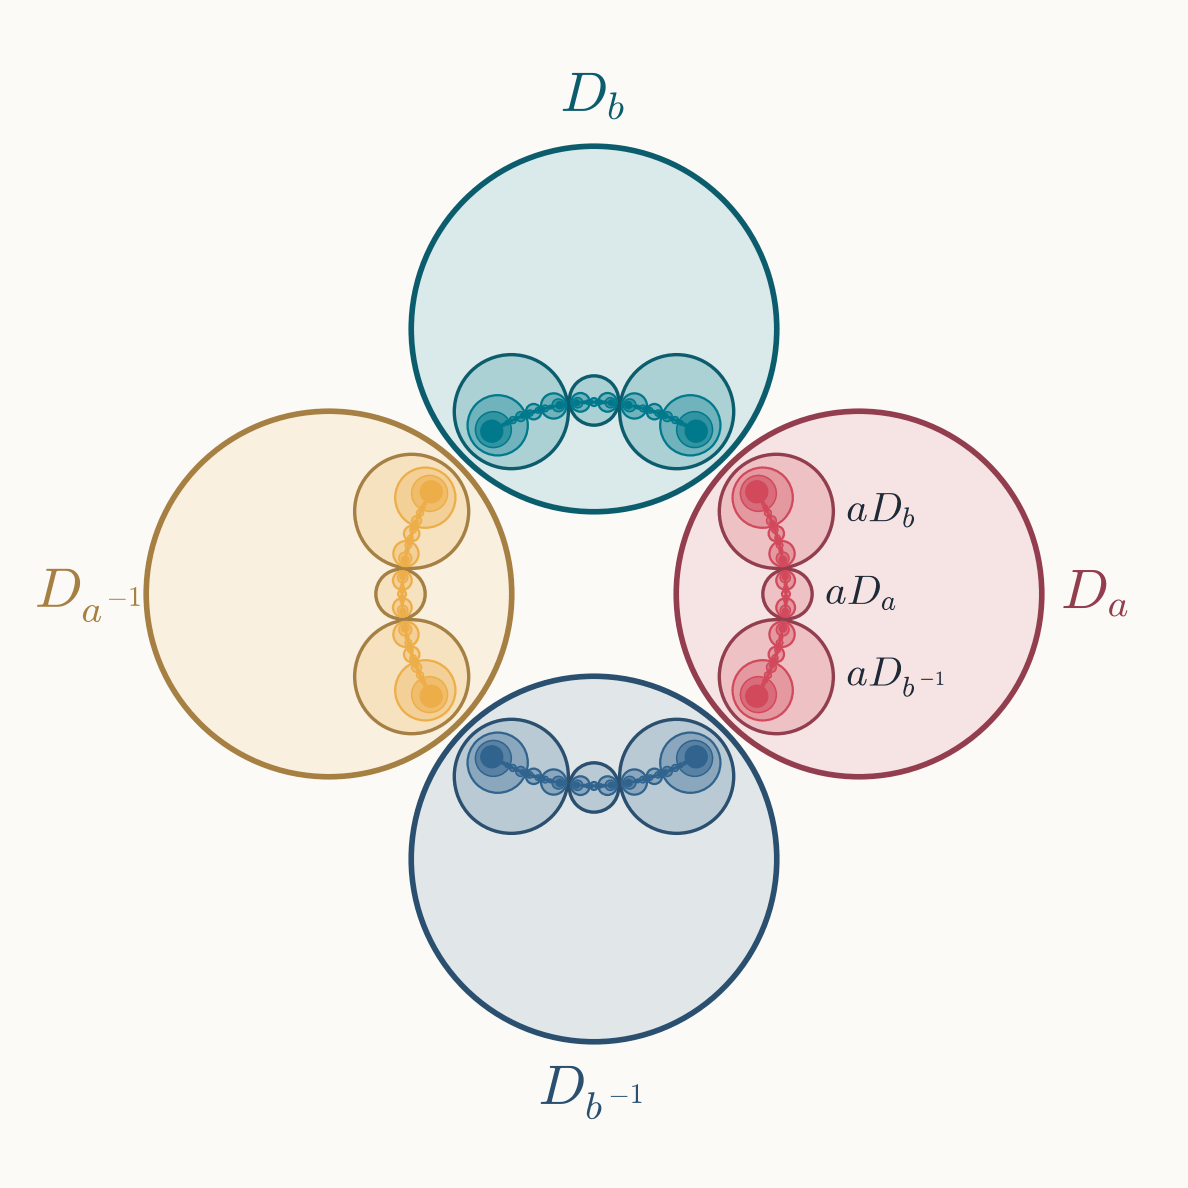
\includegraphics[width=0.48\linewidth]{schottky.png}
  \caption{A Schottky group. The discs have radius $1$ and centers $\pm 1.45$
  and $\pm 1.45i$, and \eqref{eq:pairing} gives
  $a(z) = 1.45 - 1/(z + 1.45)$ and $b(z) = 1.45i + 1/(z + 1.45i)$. Inside
  each $D_s$ are the discs $w(D_t)$ for the reduced words $wt$ of length $2$
  to $5$ that begin with $s$, darker for longer words. Here $aD_t$ means
  $a(D_t)$.}
  \label{fig:schottky}
\end{figure}

The picture is the proof of Theorem~\ref{thm:pingpong} drawn for all words
at once. If
$w = s_1 \cdots s_n$ is reduced and $t \ne s_n^{-1}$, then $w(D_t)$ is a disc
inside $D_{s_1}$. If moreover $t' \ne t^{-1}$, then
$wt(D_{t'}) \subseteq w(D_t)$, because $t(D_{t'}) \subseteq D_t$. So the discs
$w(D_t)$, one for each nonempty reduced word $wt$, are nested exactly as the
branches of the tree in Figure~\ref{fig:tree}. Call the discs with
$\abs{wt} = n$ the discs of level $n$. Discs of the same level are pairwise
disjoint, by induction on $n$, since each map is injective.

The intersection over $n$ of the unions of the closed discs of level $n$ is
the \emph{limit set} of $\gen{a,b}$. One can show that it is a Cantor set,
whose points correspond to the infinite reduced words. The closed region $F$
outside the four discs is a fundamental domain for the action on the
complement of the limit set. Gluing $\partial D_{a^{-1}}$ to $\partial D_a$
by $a$, and $\partial D_{b^{-1}}$ to $\partial D_b$ by $b$, turns $F$ into a
closed surface of genus~$2$.
